\documentclass[notheorems, handout, 10pt]{beamer}

\usetheme[numbers,totalnumbers,compress, nologo]{Statmod}
\usefonttheme[onlymath]{serif}
\setbeamertemplate{navigation symbols}{}

\mode<handout> {
	\usepackage{pgfpages}
	%\setbeameroption{show notes}
	%\pgfpagesuselayout{2 on 1}[a4paper, border shrink=5mm]
	\setbeamercolor{note page}{bg=white}
	\setbeamercolor{note title}{bg=gray!10}
	\setbeamercolor{note date}{fg=gray!10}
}

\usepackage[utf8x]{inputenc}
\usepackage[T1,T2A]{fontenc}
\usepackage[russian]{babel}

\usepackage{amsmath,amsthm,amssymb}
\usepackage{mathtext}
\usepackage{graphicx}

\title[Рекуррентные сети]{Рекуррентные сети}
\author[Самарин И.А.]{Самарин Игорь, группа 23.М03-мм}
\institute{Санкт-Петербургский государственный университет\\Кафедра статистического моделирования}
\date{\vspace{3cm}\\Санкт-Петербург\\2024 г.}

\subject{Talks}

\setbeamertemplate{caption}[numbered]

\setbeamercolor{bluetext_color}{fg=blue}
\newcommand{\bluetext}[1]{{\usebeamercolor[fg]{bluetext_color}#1}}

\begin{document}
	
	\listoftables

	\begin{frame}[plain]
		
		\titlepage
		
		\note{ 
			
		}
		
	\end{frame}
	
	\begin{frame}{Нейронная сеть. Определение}
		
		\textsl{Искусственная нейронная сеть} "--- это сложная дифференцируемая функция, задающая отображение из исходного пространства в пространство ответов, все параметры которой могут настраиваться одновременно и взаимосвязанно.
		
		\vspace{0.2cm}
		
		Сложную функцию удобно представлять в виде суперпозиции простых. Простейшие разновидности:
		\begin{itemize}
			\item \textbf{Линейный слой}: линейное преобразование над входящими данными. Обучаемые параметры "--- матрица $W$ и вектор $b$ такие, что $x \mapsto xW + b$, где $(W \in \mathbb{R}^{d\times k}, x \in \mathbb{R}^{d}, b \in \mathbb{R}^{k})$;
			\item \textbf{Функция активации}: нелинейное преобразование, поэлементно применяющееся к пришедшим на вход данным.
		\end{itemize}
		
		Таким образом, нейронную сеть можно представить в виде вычислительного графа, где промежуточным вершинам соотствуют преобразования.
		
		\note{}
	
	\end{frame}
	
	\begin{frame}{Нейронная сеть}
		
		\begin{figure}[H]
			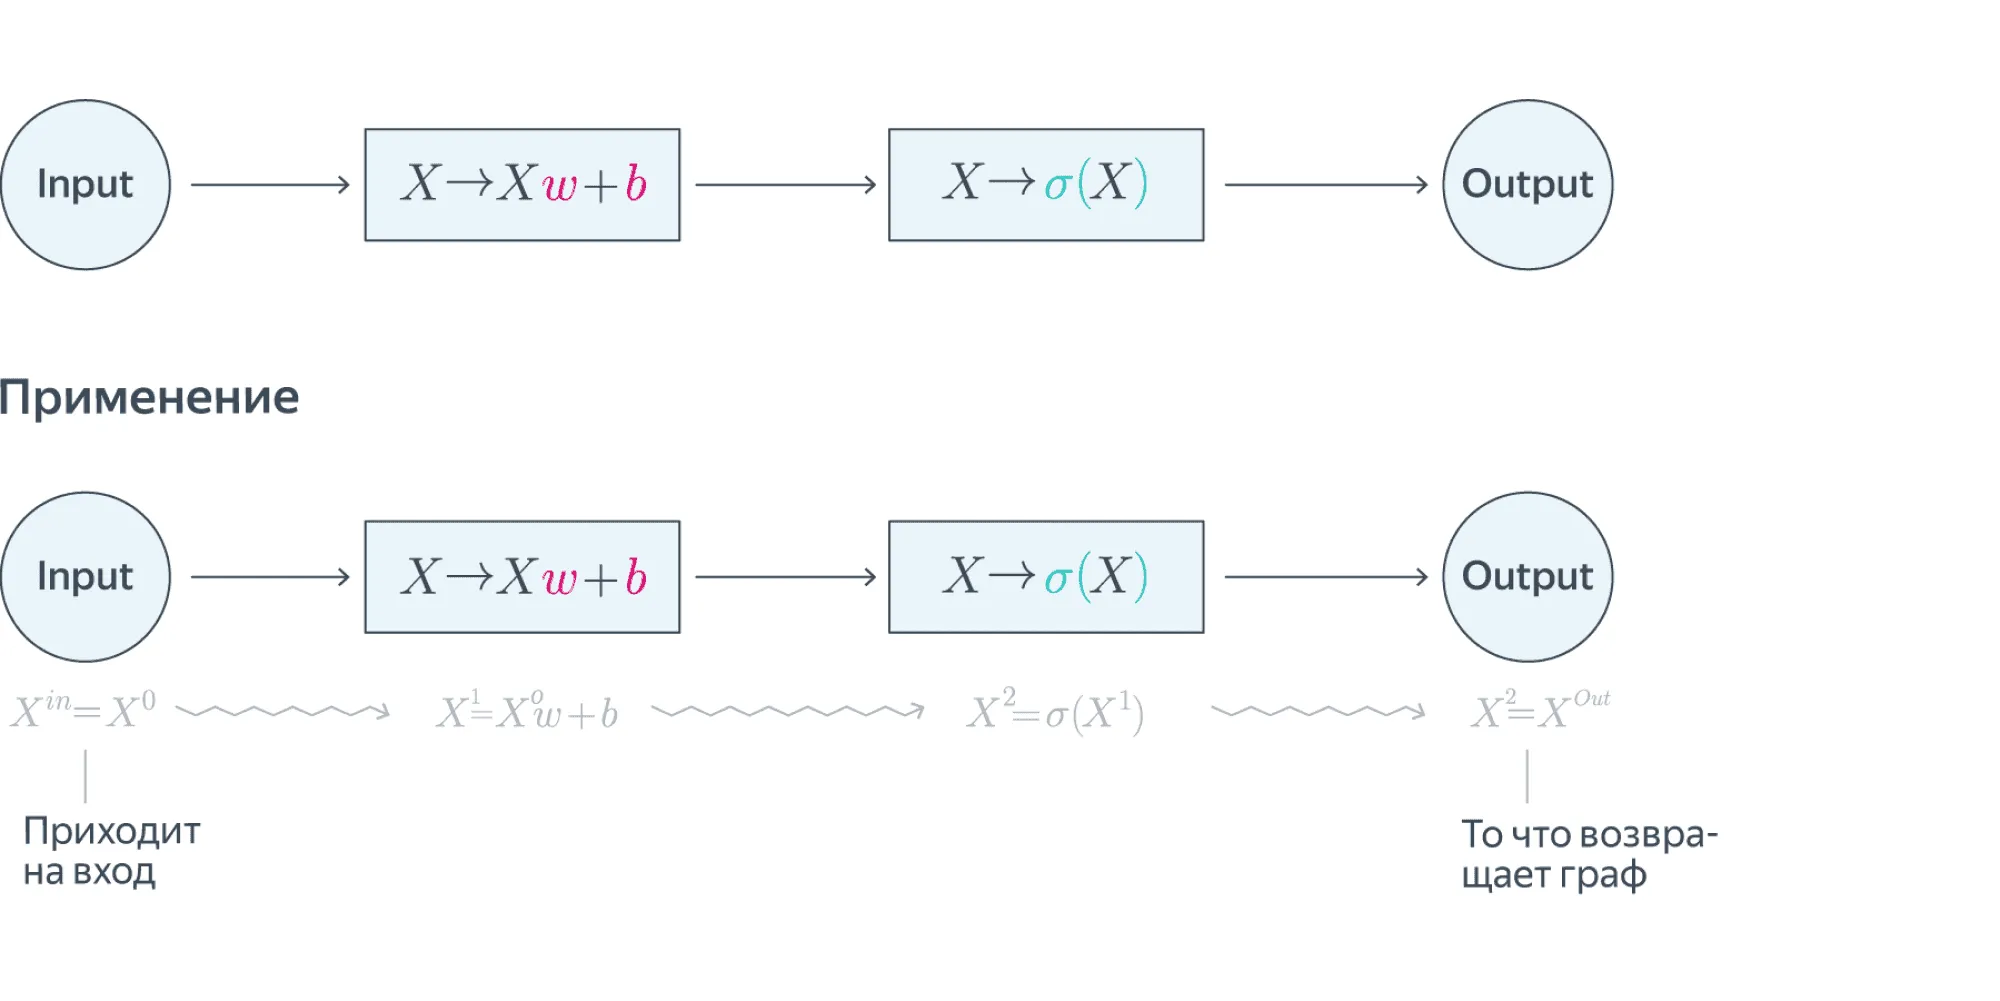
\includegraphics[width=1\linewidth]{images/1}
		\end{figure}
		
		\note{}
		
	\end{frame}
	
	\begin{frame}{Рекуррентная нейронная сеть. Мотивация}
		
		Традиционные нейронные сети не позволяют сохранять информацию и в этом их главный недостаток. 
		
		\vspace{0.5cm}
		
		В отличие от других данных временные ряды и тексты содержат временную компоненту. Поэтому хотелось бы иметь возможность обрабатывать их последовательно, в строго определенном порядке.
		
		\vspace{0.5cm}
		
		Решить эту проблему помогают рекуррентные нейронные сети. Это сети, содержащие обратные связи и позволяющие сохранять информацию.
		
		\note{}
		
	\end{frame}
	
	\begin{frame}{Рекуррентная нейронная сеть. Определение}
		
		Рекуррентная нейронная сеть "--- это вид нейронной сети, где связи между элементами образуют направленную последовательность.
		
		\begin{figure}[H]
			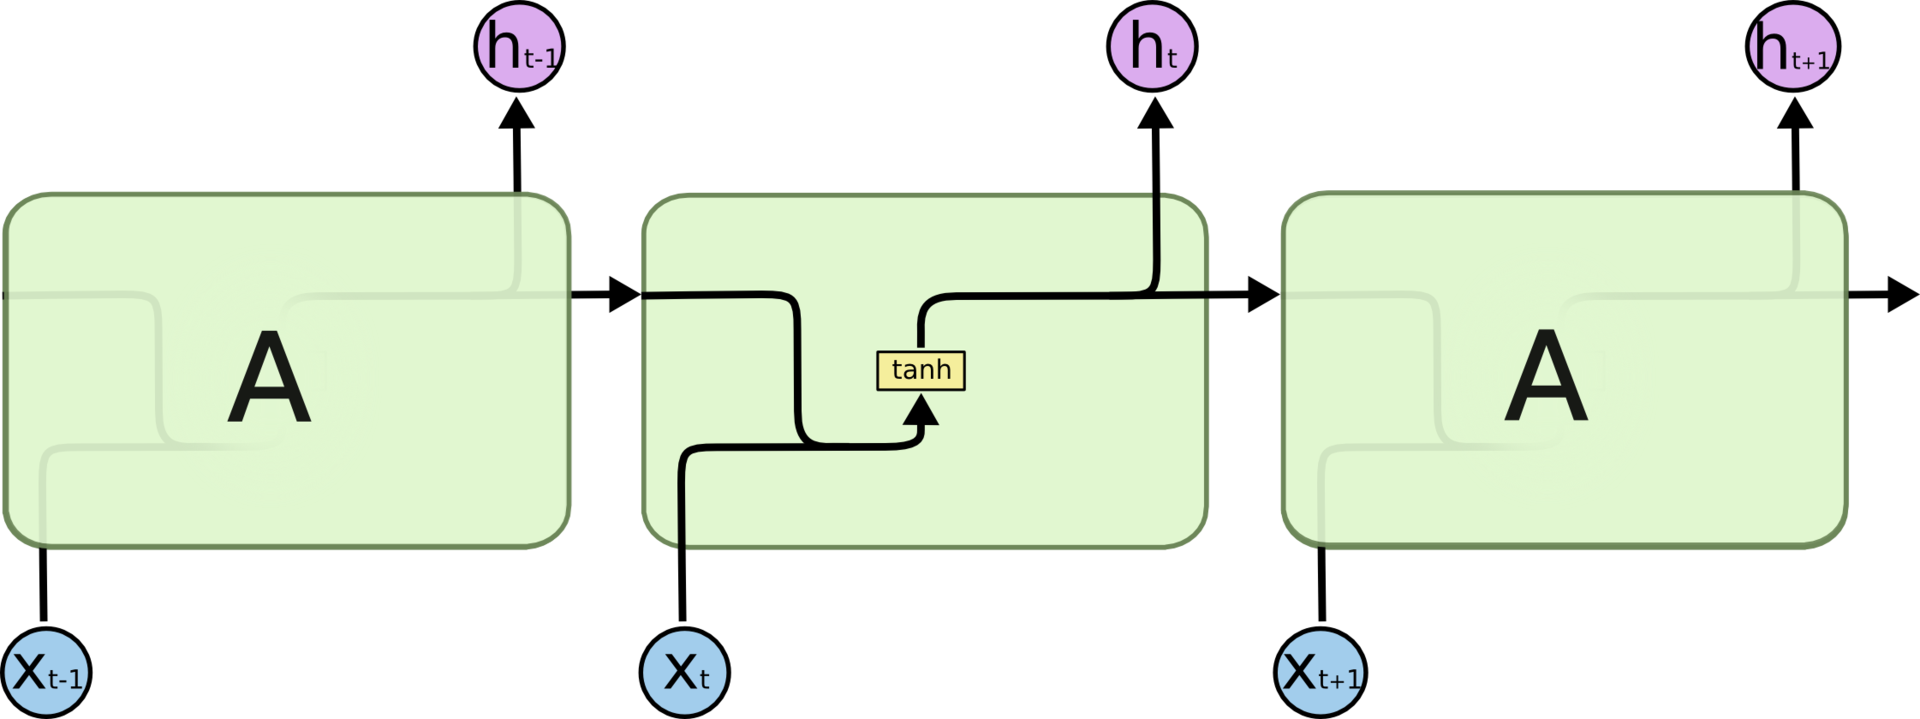
\includegraphics[width=1\linewidth]{images/5}
		\end{figure}
		
		Рекуррентные сети представимы в виде цепочки блоков. В нашем случае, повторяющимся блоком является линейный слой с гиперболическим тангенсом в качестве активации.
		
		\note{}
		
	\end{frame}
	
	\begin{frame}{Рекуррентная нейронная сеть. Скрытое состояние}
		
		Рассмотрим идею рекуррентных нейронных сетей:
		
		\begin{figure}[H]
			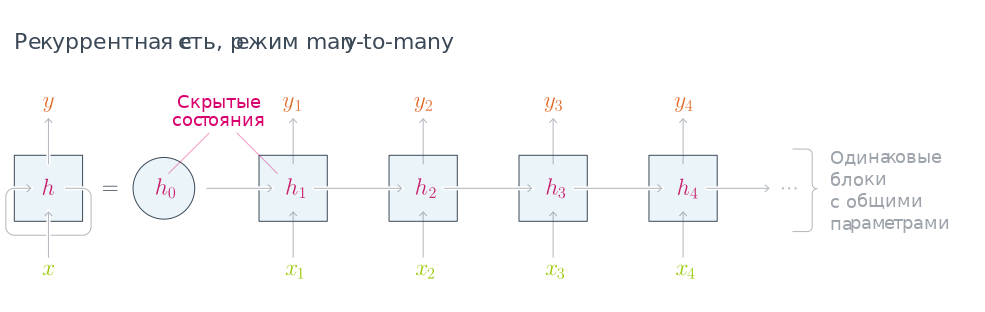
\includegraphics[width=1\linewidth]{images/3}
		\end{figure}
		
		На схеме, скрытое состояние $h$ принимает входное значение $x$ и возвращает значение $y$. Наличие обратной связи позволяет передавать информацию от одного шага сети к другому.
		
		\note{}
		
	\end{frame}
	\begin{frame}{Рекуррентная нейронная сеть. Скрытое состояние}
	
		На каждом шаге в сеть подаются данные, при этом происходит обновление скрытого состояния: $$h_n = \tanh(h_{n-1}W_1 + x_nW_2),$$ после чего, по скрытому состоянию, предсказывается выходной сигнал: $$y_n=h_nW_3,$$ где $W_i$ одинаковы на всех итерациях.
		
		\note{}
		
	\end{frame}
	
	\begin{frame}{Двунаправленная рекуррентная нейронная сеть}
		
		Двунаправленная рекуррентная нейронная сеть позволяет учитывать не только предыдущие значения, но и последующие.
		
		\begin{figure}[H]
			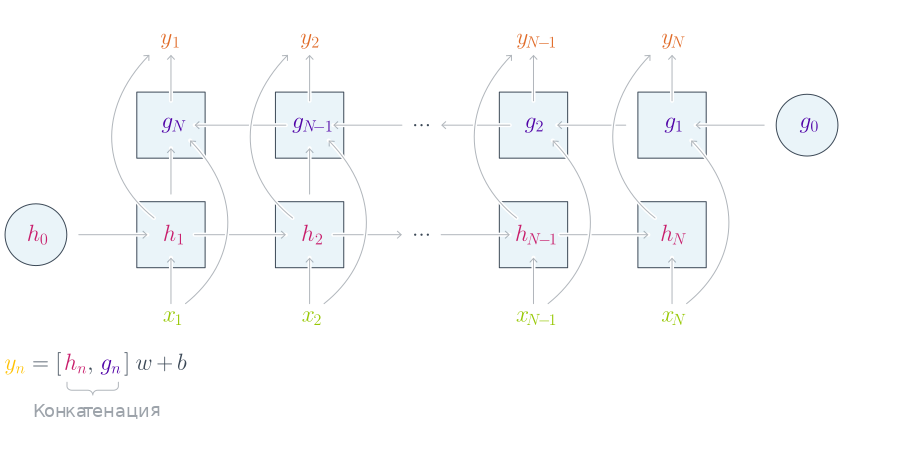
\includegraphics[width=1\linewidth]{images/4}
		\end{figure}
		
		Формула для $y_n$ может быть другой. Например, выходы сетей могут агрегироваться путем усреднения, или любым другим способом.
		
		\note{}
		
	\end{frame}
	
	\begin{frame}{Взрыв и затухание градиента}
		
		Рассмотрим функцию потерь $\mathfrak{L}_n=L(y_n, \hat{y}_n)$, измеряющую отклонение $n$-го выхода от истинного. Выход $y_n$ зависит от скрытого состояния $h_n$, а тот, в свою очередь, от всех $h_i$, $i < n$.
		
		\vspace{0.5cm}
		
		Обновление градиента при $h_i=\tanh(h_{i-1}W_1 + x_iW_2)$ будет иметь вид: $$\nabla_{h_{i-1}}L=(\nabla_{h_{i-1}L}W_1^T \cdot \tanh'(h_{i-1}W_1 + x_iW_2)),$$ т.е. в ходе вычисления $\nabla_{W_1}\mathfrak{L}_n$ мы $(n-1)$ раз будем умножать на $W_1^T$. Если у нее есть с.з., по модулю большие 1, градиент будет стремиться к бесконечности (взрываться).
		
		\vspace{0.5cm}
		
		Вариант решения: gradient clipping "--- заменять значения градиента выше некоторого порога на некоторую константу.
		
		\note{}
		
	\end{frame}
	
	\begin{frame}{LSTM}
		
		Сеть с долговременной и кратковременной памятью частично решает проблему взрыва и затухания градиента.
		
		\begin{figure}[H]
			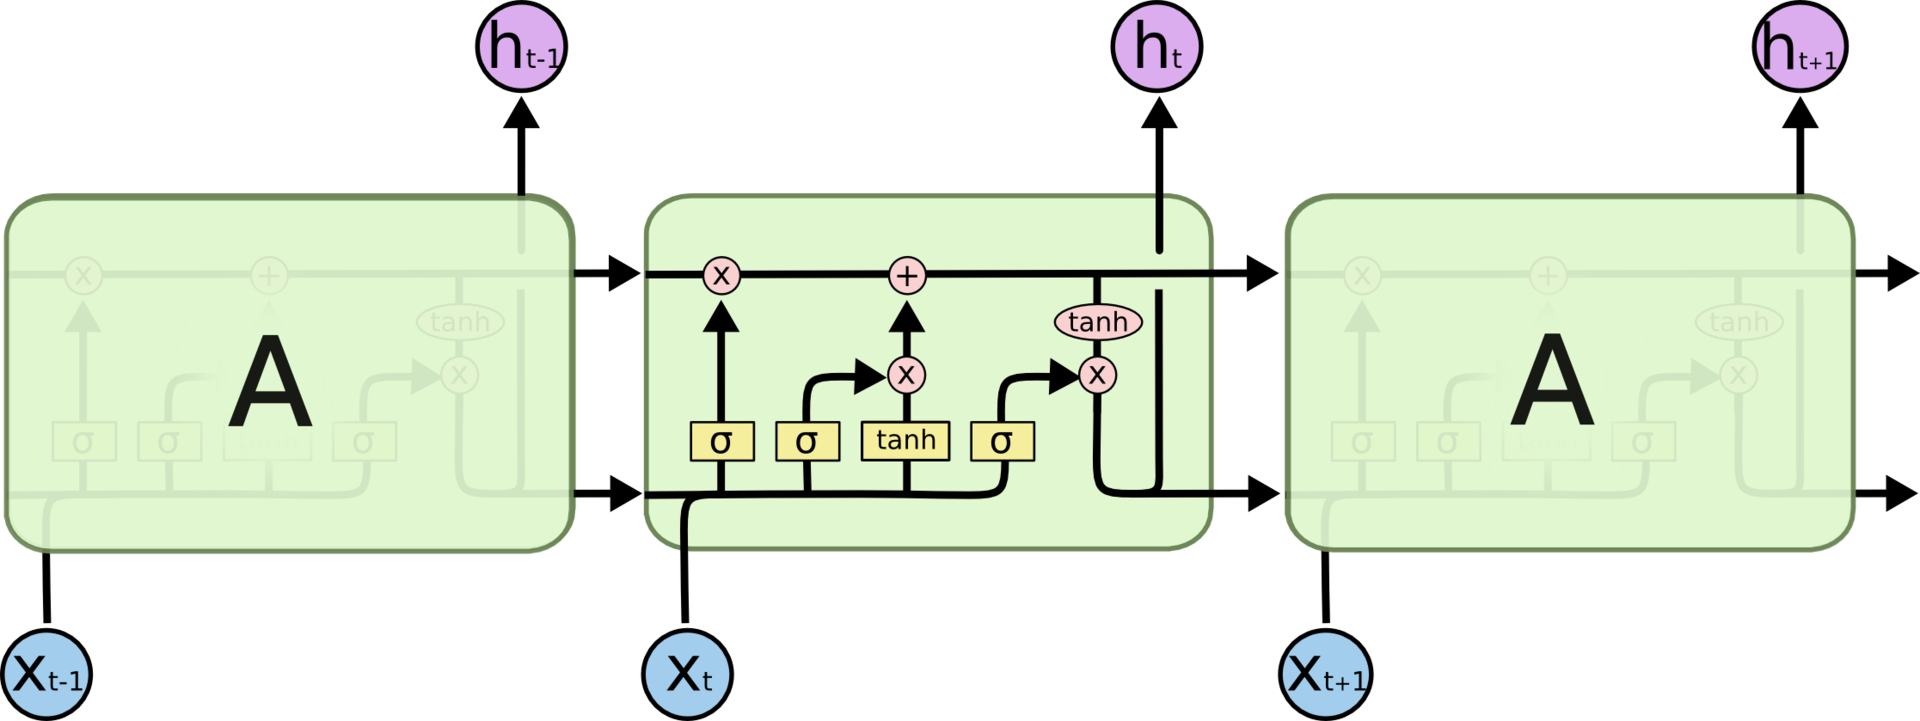
\includegraphics[width=1\linewidth]{images/6}
		\end{figure}
		
		Рассмотрим механизм подробнее.
		
		\note{}
		
	\end{frame}
	
	\begin{frame}{LSTM. Состояние блока}
		
		Помимо скрытого состояния $h_n$, появляется понятие cell state $c_n$.
		
		\vspace{0.5cm}
		
		Cell state играет роль внутренней, закрытой информации LSTM блока, тогда как скрытое состояние становится значением передаваемым наружу.
		
		\vspace{0.5cm}
		
		LSTM может добавлять или удалять информацию из cell state с помощью вентилей.
	
		\note{}
		
	\end{frame}
	
	\begin{frame}{LSTM. Забывание информации}
		
		Вентиль забывания, по предыдущему скрытому состоянию $h_{t-1}$ и входу $x_t$, позволяет определить, какую долю информации из $c_{n-1}$ стоит пропустить, а какую забыть.
		
		\begin{figure}[H]
			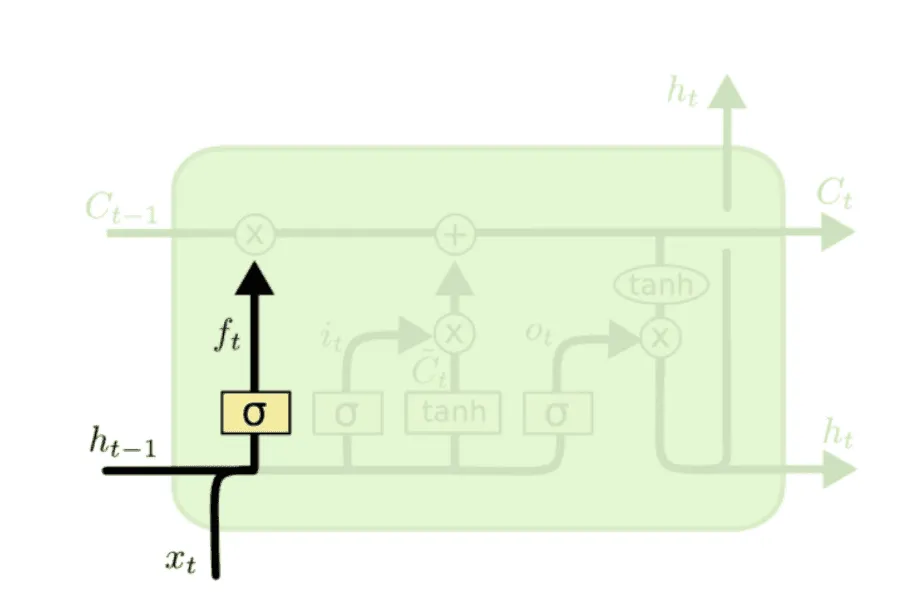
\includegraphics[width=0.5\linewidth]{images/7}
		\end{figure}
		
		Доля $f_t$ сохраняемой информации из $c_{t-1}$ вычисляется: $$f_t=\sigma(h_{t-1}W_1^f + x_tW_2^f+b_f).$$
		
		\note{}
		
	\end{frame}
	
	\begin{frame}{LSTM. Сохранение информации}
		
		Необходимо определить, чего нового мы внесем в cell state. Для этого вычисляем: $$\tilde{c}_t = \tanh(h_{t-1}W_1^c+x_tW_2^c+b_c).$$ 
		
		\begin{figure}[H]
			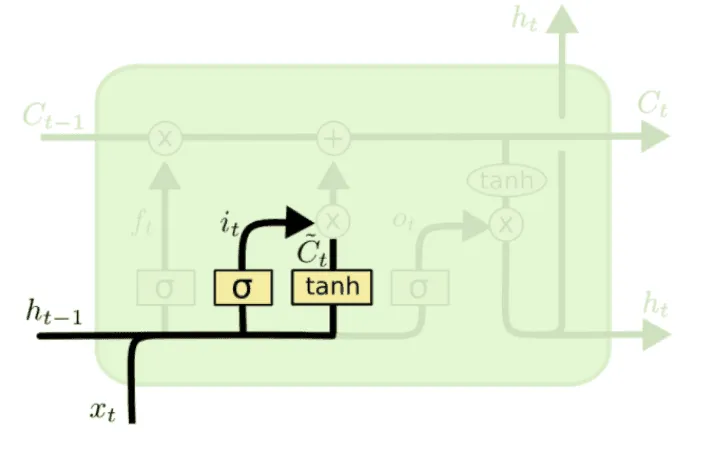
\includegraphics[width=0.5\linewidth]{images/8}
		\end{figure}
		
		Однако, мы не уверены, что вся информация достойна переноса в cell state, поэтому хотим взять лишь долю.
		
		\note{}
		
	\end{frame}
	
	\begin{frame}{LSTM. Сохранение информации}
		
		Вентиль входного состояния позволяет определить, какую долю релевантной информации стоит сохранить.
		
		\begin{figure}[H]
			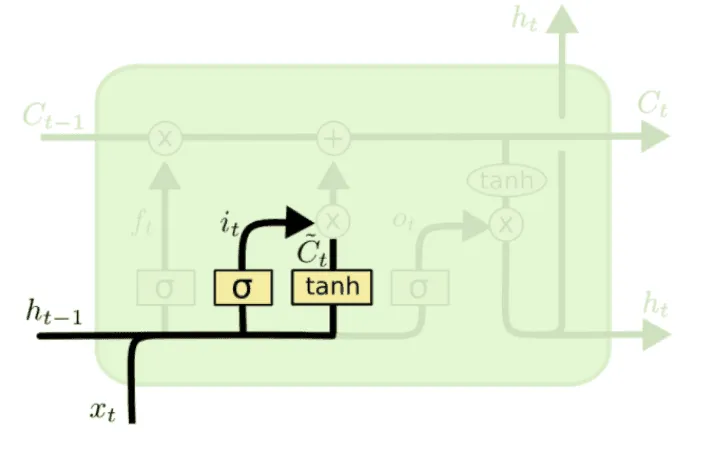
\includegraphics[width=0.5\linewidth]{images/8}
		\end{figure}
		
		Доля $i_t$ сохраняемой информации вычисляется: $$i_t=\sigma(h_{t-1}W_1^i+x_tW_2^i+b_i).$$
	
		\note{}
		
	\end{frame}
	
	\begin{frame}{LSTM. Новое состояние блока}
		
		Новое состояние блока вычисляется: $$c_t=f_t\cdot c_{t-1} + i_t \cdot \tilde{c}_t,$$ где $\cdot$ "--- это поэлементное умножение. 
	
		\begin{figure}[H]
			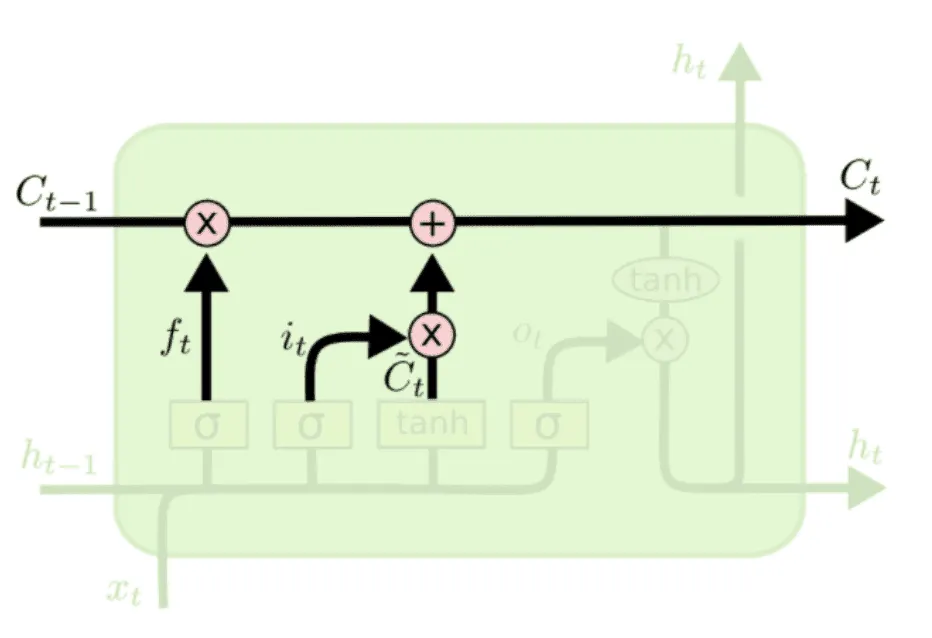
\includegraphics[width=0.5\linewidth]{images/9}
		\end{figure}
		
		Первое слагаемое отвечает за забывание информации из $c_{t-1}$, а второе "--- за запоминание новой.
		
		\note{}
		
	\end{frame}
	
	\begin{frame}{LSTM. Выходное значение}
		
		Вентиль выходного состояния позволяет определить, сколько информации следует отдать на выход. Доля вычисляется: $$o_t=\sigma(h_{t-1}W_1^o + x_tW_2^o +b_o).$$
		
		\begin{figure}[H]
			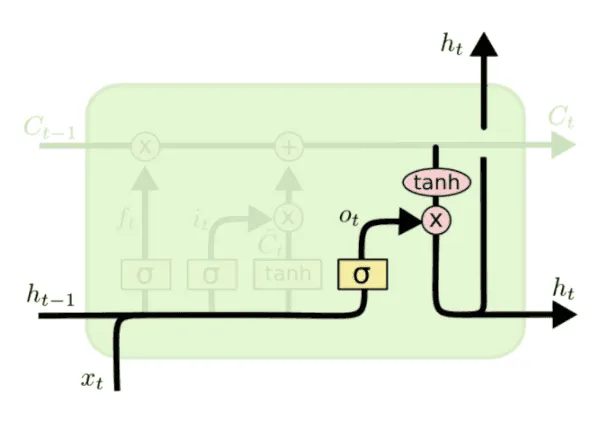
\includegraphics[width=0.5\linewidth]{images/10}
		\end{figure}
		
		Чтобы отфильтровать информацию из cell state, вычисляем: $$h_t=o_t \cdot \tanh(c_t).$$
		
		\note{}
		
	\end{frame}
	
	\begin{frame}{GRU}
		
		Вычисление четырех гейтов может быть вычислительно трудным, поэтому иногда используют GRU.
		
		\begin{figure}[H]
			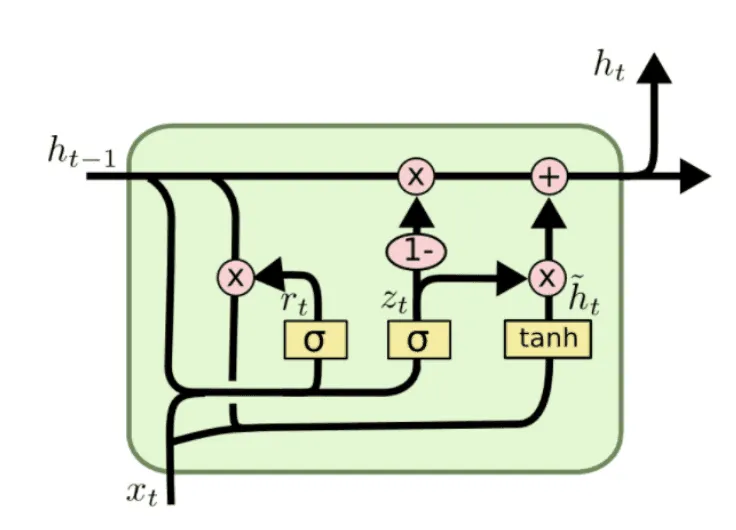
\includegraphics[width=0.5\linewidth]{images/11}
		\end{figure}
		
		GRU объединяет input gate и forget gate в один update gate, а также устраняет разделение на hidden и cell state.
		
		\note{}
		
	\end{frame}
	
	\begin{frame}{GRU}
		
		В итоге GRU имеет меньше параметров и быстрее учится. 
		
		\vspace{0.5cm}
		
		Более того, GRU и LSTM показывают сопостовимое качество на многих задачах обработки естественного языка и генерации музыки.
		
		\note{}
		
	\end{frame}
	
\end{document}